\documentclass[11pt, a4paper]{article}\usepackage[]{graphicx}\usepackage[]{xcolor}
% maxwidth is the original width if it is less than linewidth
% otherwise use linewidth (to make sure the graphics do not exceed the margin)
\makeatletter
\def\maxwidth{ %
  \ifdim\Gin@nat@width>\linewidth
    \linewidth
  \else
    \Gin@nat@width
  \fi
}
\makeatother

\definecolor{fgcolor}{rgb}{0.345, 0.345, 0.345}
\newcommand{\hlnum}[1]{\textcolor[rgb]{0.686,0.059,0.569}{#1}}%
\newcommand{\hlsng}[1]{\textcolor[rgb]{0.192,0.494,0.8}{#1}}%
\newcommand{\hlcom}[1]{\textcolor[rgb]{0.678,0.584,0.686}{\textit{#1}}}%
\newcommand{\hlopt}[1]{\textcolor[rgb]{0,0,0}{#1}}%
\newcommand{\hldef}[1]{\textcolor[rgb]{0.345,0.345,0.345}{#1}}%
\newcommand{\hlkwa}[1]{\textcolor[rgb]{0.161,0.373,0.58}{\textbf{#1}}}%
\newcommand{\hlkwb}[1]{\textcolor[rgb]{0.69,0.353,0.396}{#1}}%
\newcommand{\hlkwc}[1]{\textcolor[rgb]{0.333,0.667,0.333}{#1}}%
\newcommand{\hlkwd}[1]{\textcolor[rgb]{0.737,0.353,0.396}{\textbf{#1}}}%
\let\hlipl\hlkwb

\usepackage{framed}
\makeatletter
\newenvironment{kframe}{%
 \def\at@end@of@kframe{}%
 \ifinner\ifhmode%
  \def\at@end@of@kframe{\end{minipage}}%
  \begin{minipage}{\columnwidth}%
 \fi\fi%
 \def\FrameCommand##1{\hskip\@totalleftmargin \hskip-\fboxsep
 \colorbox{shadecolor}{##1}\hskip-\fboxsep
     % There is no \\@totalrightmargin, so:
     \hskip-\linewidth \hskip-\@totalleftmargin \hskip\columnwidth}%
 \MakeFramed {\advance\hsize-\width
   \@totalleftmargin\z@ \linewidth\hsize
   \@setminipage}}%
 {\par\unskip\endMakeFramed%
 \at@end@of@kframe}
\makeatother

\definecolor{shadecolor}{rgb}{.97, .97, .97}
\definecolor{messagecolor}{rgb}{0, 0, 0}
\definecolor{warningcolor}{rgb}{1, 0, 1}
\definecolor{errorcolor}{rgb}{1, 0, 0}
\newenvironment{knitrout}{}{} % an empty environment to be redefined in TeX

\usepackage{alltt}

\usepackage[top = 1 in, bottom = 1 in, left = 1 in, right = 1 in ]{geometry}

\usepackage{amsmath, amssymb, amsfonts}
\usepackage{enumerate}
\usepackage{array}
\usepackage{multirow}
\usepackage{dingbat}
\usepackage{fontawesome5}
\usepackage{tasks}
\usepackage{bbding}
\usepackage{undertilde}
\usepackage{twemojis}
\usepackage{simpsons}
% how to use bull's eye ----- \scalebox{2.0}{\twemoji{bullseye}}
\usepackage{fontspec}
\usepackage{customdice}
% how to put dice face ------ \dice{2}

\title{MSMS 206 : Practical 09}
\author{Ananda Biswas}
\date{\today}

\newfontface\myfont{Myfont1-Regular.ttf}[LetterSpace=0.05em]
% how to use ---- {\setlength{\spaceskip}{1em plus 0.5em minus 0.5em} \fontsize{17}{20}\myfont --write text here-- \par}

\newfontface\cbfont{CaveatBrush-Regular.ttf}
% how to use --- \myfont --write text here--
\IfFileExists{upquote.sty}{\usepackage{upquote}}{}
\begin{document}

\maketitle


\scalebox{2.0}{\twemoji{bullseye}} \hspace{0.2cm} \textcolor{blue}{\textbf{Question : }} Fit a decision tree model using the \textbf{Loan Defaulters' Dataset} given as follows :

\begin{table}[!htbp]
\def\arraystretch{1.5}

\begin{center}
\begin{tabular}{|>{\centering}m{3cm}|>{\centering}m{3cm}|>{\centering}m{3cm}|>{\centering\arraybackslash}m{5cm}|}

\hline

\textbf{Home Owner} & \textbf{Married Status} & \textbf{Defaulted} & \textbf{Annual Income(\$)} \\

\hline

yes & single    & no  & 125000 \\

\hline

no  & married   & no  & 100000 \\

\hline

no  & single    & no  &  70000 \\

\hline

yes & married   & no  & 120000 \\

\hline

no  & divorcee  & yes &  95000 \\

\hline

no  & married   & no  &  60000 \\

\hline

yes & divorcee  & no  & 220000 \\

\hline

no  & single    & yes &  85000 \\

\hline

no  & married   & no  &  75000 \\

\hline

no  & single    & yes &  90000 \\

\hline

\end{tabular}
\end{center}
\end{table}

Will a divorcee home owner with annual income \$120000 default in his loan ? \\[1.5em]

\faArrowAltCircleRight[regular] \hspace{0.2cm} \underline{Building Decision Tree Model}

\begin{knitrout}
\definecolor{shadecolor}{rgb}{0.969, 0.969, 0.969}\color{fgcolor}\begin{kframe}
\begin{alltt}
\hlkwd{library}\hldef{(rpart)}
\hlkwd{library}\hldef{(rpart.plot)}
\end{alltt}
\end{kframe}
\end{knitrout}

\begin{knitrout}\tiny
\definecolor{shadecolor}{rgb}{0.969, 0.969, 0.969}\color{fgcolor}\begin{kframe}
\begin{alltt}
\hldef{df} \hlkwb{<-} \hlkwd{read.csv}\hldef{(}\hlsng{'https://raw.githubusercontent.com/sakunisgithub/data_sets/refs/heads/master/msc_semester_2/loan_defaulter_data.csv'}\hldef{)}
\end{alltt}
\end{kframe}
\end{knitrout}

\newpage

\begin{knitrout}
\definecolor{shadecolor}{rgb}{0.969, 0.969, 0.969}\color{fgcolor}\begin{kframe}
\begin{alltt}
\hldef{tree_model} \hlkwb{<-} \hlkwd{rpart}\hldef{(Defaulted} \hlopt{~} \hldef{.,}
                    \hlkwc{data} \hldef{= df,}
                    \hlkwc{method} \hldef{=} \hlsng{"class"}\hldef{,}
                    \hlkwc{parms} \hldef{=} \hlkwd{list}\hldef{(}\hlkwc{split} \hldef{=} \hlsng{"information"}\hldef{),}
                    \hlkwc{control} \hldef{=} \hlkwd{rpart.control}\hldef{(}\hlkwc{minsplit} \hldef{=} \hlnum{2}\hldef{,}
                                            \hlkwc{minbucket} \hldef{=} \hlnum{1}\hldef{,}
                                            \hlkwc{cp} \hldef{=} \hlnum{0.01}\hldef{))}
\end{alltt}
\end{kframe}
\end{knitrout}

\begin{knitrout}
\definecolor{shadecolor}{rgb}{0.969, 0.969, 0.969}\color{fgcolor}\begin{kframe}
\begin{alltt}
\hlkwd{print}\hldef{(tree_model)}
\end{alltt}
\begin{verbatim}
## n= 10 
## 
## node), split, n, loss, yval, (yprob)
##       * denotes terminal node
## 
##  1) root 10 3 no (0.7000000 0.3000000)  
##    2) Married_Status=married 4 0 no (1.0000000 0.0000000) *
##    3) Married_Status=divorcee,single 6 3 no (0.5000000 0.5000000)  
##      6) Home_Owner=yes 2 0 no (1.0000000 0.0000000) *
##      7) Home_Owner=no 4 1 yes (0.2500000 0.7500000)  
##       14) Annual_Income< 77500 1 0 no (1.0000000 0.0000000) *
##       15) Annual_Income>=77500 3 0 yes (0.0000000 1.0000000) *
\end{verbatim}
\end{kframe}
\end{knitrout}

\newpage

\faArrowAltCircleRight[regular] \hspace{0.2cm} \underline{Visualizing the Decision Tree Model}

\begin{knitrout}
\definecolor{shadecolor}{rgb}{0.969, 0.969, 0.969}\color{fgcolor}\begin{kframe}
\begin{alltt}
\hlkwd{rpart.plot}\hldef{(tree_model,}
           \hlkwc{type} \hldef{=} \hlnum{5}\hldef{,}
           \hlkwc{extra} \hldef{=} \hlnum{0}\hldef{,}
           \hlkwc{box.palette} \hldef{=} \hlkwd{c}\hldef{(}\hlsng{"#93fd9e"}\hldef{,} \hlsng{"#fd939d"}\hldef{))}
\end{alltt}
\end{kframe}
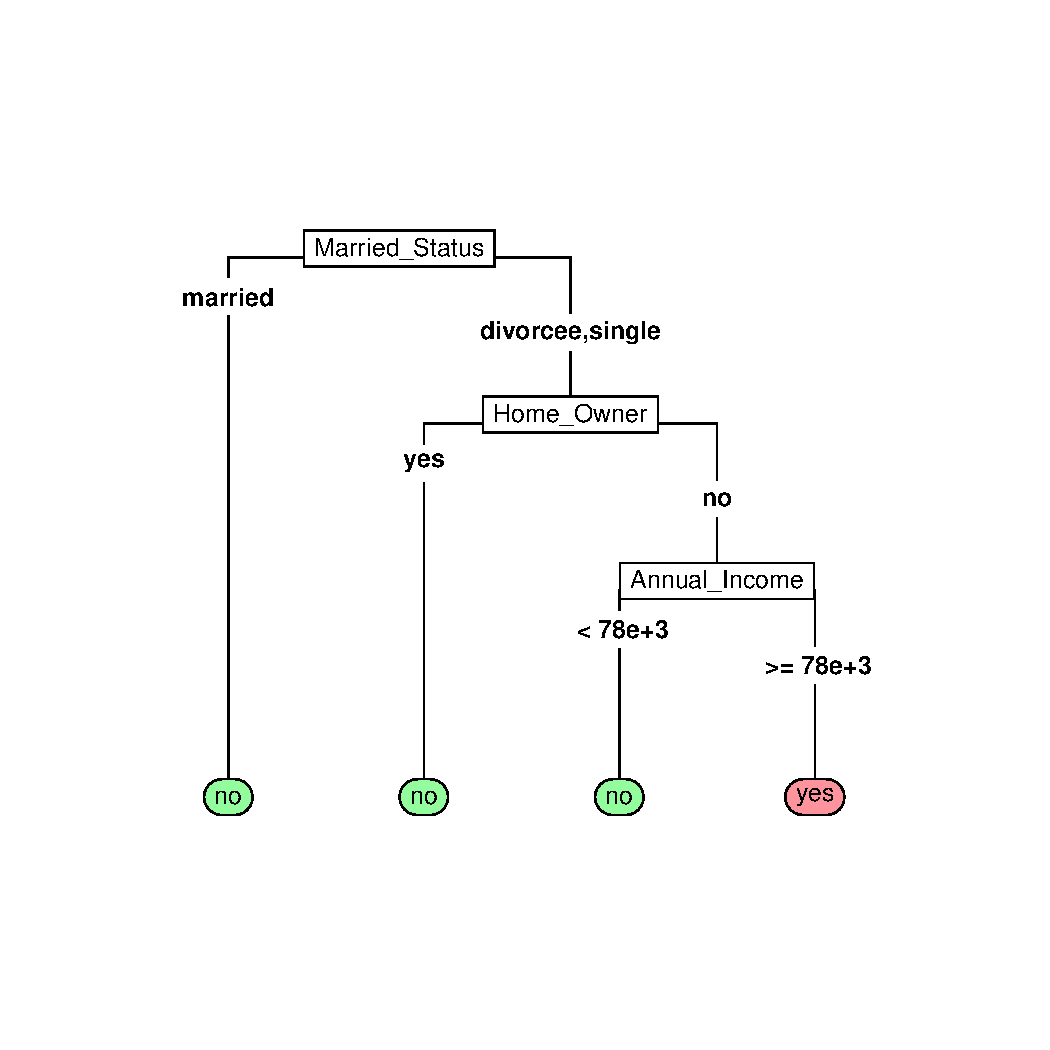
\includegraphics[width=\maxwidth]{figure/unnamed-chunk-5-1} 
\end{knitrout}

\newpage

The following diagram displays labels at all nodes, giving a comprehensive idea how the tree was made.

\begin{knitrout}
\definecolor{shadecolor}{rgb}{0.969, 0.969, 0.969}\color{fgcolor}\begin{kframe}
\begin{alltt}
\hlkwd{rpart.plot}\hldef{(tree_model,}
           \hlkwc{type} \hldef{=} \hlnum{4}\hldef{,}
           \hlkwc{extra} \hldef{=} \hlnum{104}\hldef{,}
           \hlkwc{clip.right.labs} \hldef{=} \hlnum{FALSE}\hldef{,}
           \hlkwc{box.palette} \hldef{=} \hlkwd{c}\hldef{(}\hlsng{"#93fd9e"}\hldef{,} \hlsng{"#fd939d"}\hldef{))}
\end{alltt}
\end{kframe}
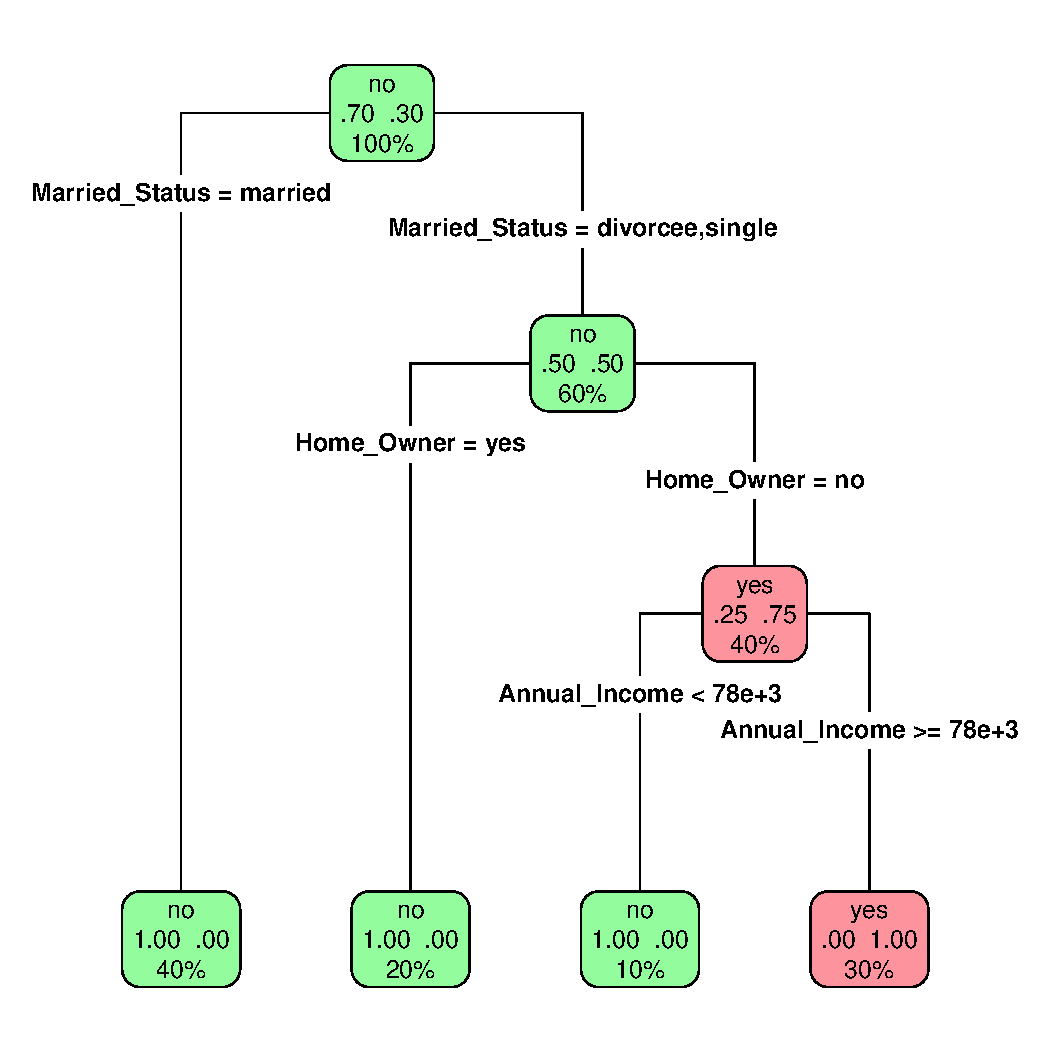
\includegraphics[width=\maxwidth]{figure/unnamed-chunk-6-1} 
\end{knitrout}

\newpage

\faArrowAltCircleRight[regular] \hspace{0.2cm} \underline{Prediction on New Example}

\begin{knitrout}
\definecolor{shadecolor}{rgb}{0.969, 0.969, 0.969}\color{fgcolor}\begin{kframe}
\begin{alltt}
\hldef{new_example} \hlkwb{<-} \hlkwd{data.frame}\hldef{(}\hlkwc{Home_Owner} \hldef{=} \hlsng{"yes"}\hldef{,}
                          \hlkwc{Married_Status} \hldef{=} \hlsng{"divorcee"}\hldef{,}
                          \hlkwc{Annual_Income} \hldef{=} \hlnum{120000}\hldef{)}
\end{alltt}
\end{kframe}
\end{knitrout}

\begin{knitrout}
\definecolor{shadecolor}{rgb}{0.969, 0.969, 0.969}\color{fgcolor}\begin{kframe}
\begin{alltt}
\hlkwd{predict}\hldef{(tree_model, new_example)}
\end{alltt}
\begin{verbatim}
##   no yes
## 1  1   0
\end{verbatim}
\end{kframe}
\end{knitrout}

{\setlength{\spaceskip}{1em plus 0.5em minus 0.5em} \fontsize{17}{20}\myfont Our decision tree model predicts that a divorcee home owner with annual income 120000 dollars will not default in his loan. \par}

\end{document}
